\documentclass[tikz,border=10pt]{standalone}
\usepackage{tikz}
\usetikzlibrary{shapes,arrows,positioning,fit,backgrounds,calc,shadows}
\usepackage{xcolor}

\definecolor{usercolor}{RGB}{44,160,44}
\definecolor{llmcolor}{RGB}{31,119,180}
\definecolor{proxycolor}{RGB}{255,127,14}
\definecolor{toolcolor}{RGB}{148,103,189}
\definecolor{provcolor}{RGB}{23,190,207}
\definecolor{policycolor}{RGB}{214,39,40}

\begin{document}
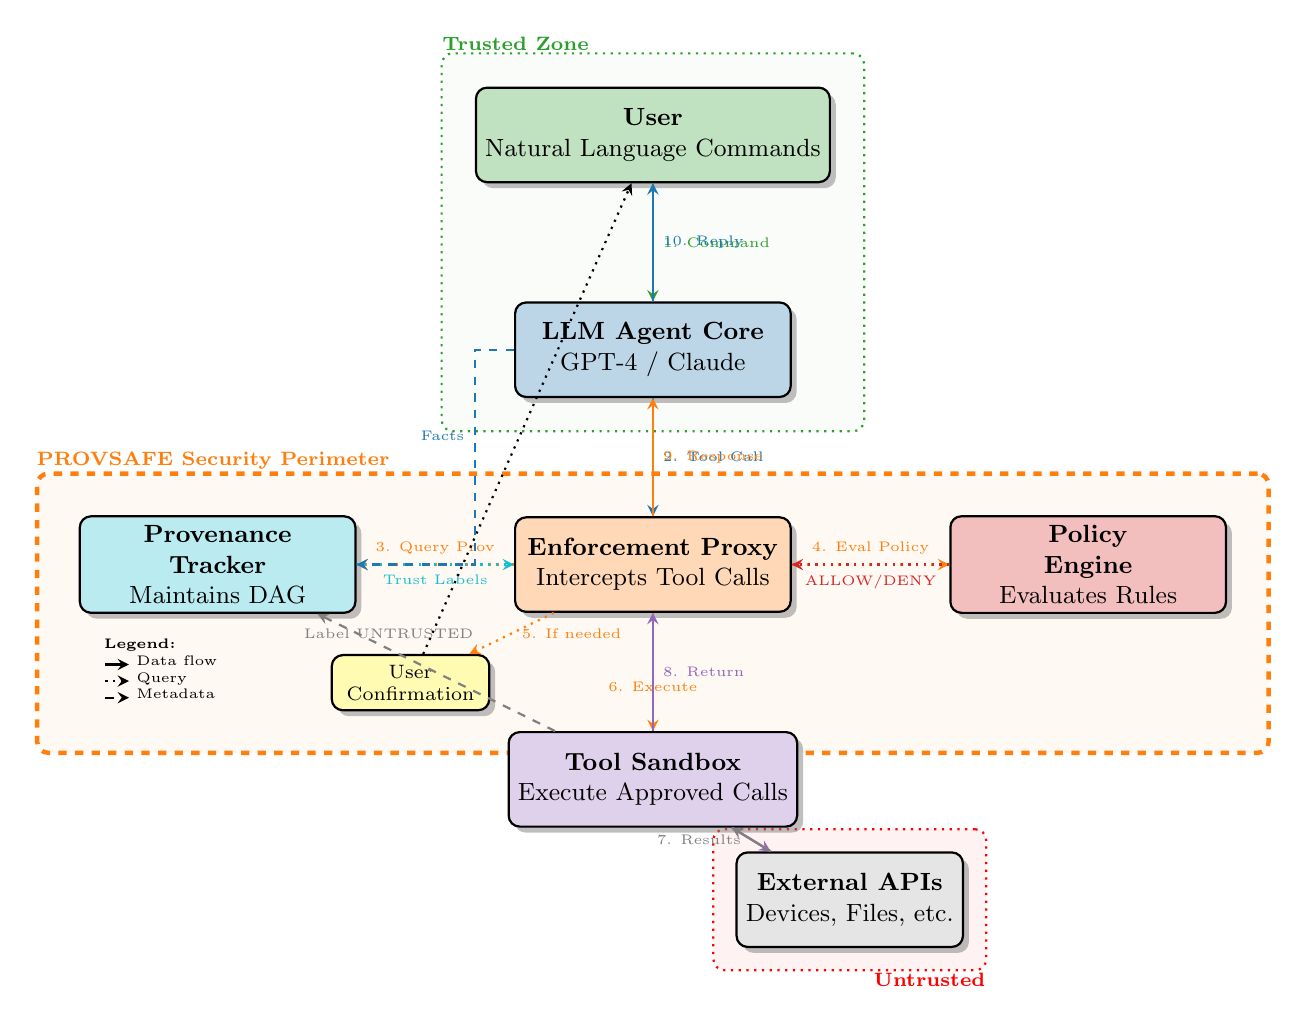
\begin{tikzpicture}[
    node distance=1cm and 1.5cm,
    every node/.style={font=\small},
    component/.style={rectangle, rounded corners, draw=black, thick, minimum width=3.5cm, minimum height=1.2cm, align=center, drop shadow},
    usercomp/.style={component, fill=usercolor!30},
    llmcomp/.style={component, fill=llmcolor!30},
    proxycomp/.style={component, fill=proxycolor!30},
    provcomp/.style={component, fill=provcolor!30},
    policycomp/.style={component, fill=policycolor!30},
    toolcomp/.style={component, fill=toolcolor!30},
    arrow/.style={->, thick, >=stealth},
    data/.style={arrow, dashed},
    query/.style={arrow, dotted, thick}
]

% Top layer: User
\node[usercomp] (user) {
    \textbf{User} \\
    Natural Language Commands
};

% LLM Agent Core
\node[llmcomp, below=1.5cm of user] (llm) {
    \textbf{LLM Agent Core} \\
    GPT-4 / Claude
};

% Enforcement Proxy (center)
\node[proxycomp, below=1.5cm of llm] (proxy) {
    \textbf{Enforcement Proxy} \\
    Intercepts Tool Calls
};

% Provenance Tracker (left)
\node[provcomp, left=2cm of proxy] (prov) {
    \textbf{Provenance} \\
    \textbf{Tracker} \\
    Maintains DAG
};

% Policy Engine (right)
\node[policycomp, right=2cm of proxy] (policy) {
    \textbf{Policy} \\
    \textbf{Engine} \\
    Evaluates Rules
};

% Tool Sandbox (bottom)
\node[toolcomp, below=1.5cm of proxy] (tools) {
    \textbf{Tool Sandbox} \\
    Execute Approved Calls
};

% External Sources (bottom right)
\node[component, fill=gray!20, below=0.3cm of tools, xshift=2.5cm, minimum width=2.5cm] (external) {
    \textbf{External APIs} \\
    Devices, Files, etc.
};

% User confirmation (left of proxy)
\node[component, fill=yellow!30, left=0.3cm of proxy, yshift=-1.5cm, minimum width=2cm, minimum height=0.7cm, font=\scriptsize] (confirm) {
    User \\
    Confirmation
};

% Main data flow arrows
\draw[arrow, usercolor] (user) -- node[right, font=\tiny] {1. Command} (llm);
\draw[arrow, llmcolor] (llm) -- node[right, font=\tiny] {2. Tool Call} (proxy);
\draw[arrow, proxycolor] (proxy) -- node[below, font=\tiny] {6. Execute} (tools);
\draw[arrow, toolcolor] (tools) -- (external);
\draw[arrow, gray] (external) -- node[left, font=\tiny] {7. Results} (tools);
\draw[arrow, toolcolor] (tools) -- node[right, font=\tiny] {8. Return} (proxy);
\draw[arrow, proxycolor] (proxy) -- node[right, font=\tiny] {9. Response} (llm);
\draw[arrow, llmcolor] (llm) -- node[right, font=\tiny] {10. Reply} (user);

% Query arrows (dashed/dotted)
\draw[query, proxycolor] (proxy) -- node[above, font=\tiny] {3. Query Prov} (prov);
\draw[query, provcolor] (prov) -- node[below, font=\tiny] {Trust Labels} (proxy);

\draw[query, proxycolor] (proxy) -- node[above, font=\tiny] {4. Eval Policy} (policy);
\draw[query, policycolor] (policy) -- node[below, font=\tiny] {ALLOW/DENY} (proxy);

% User confirmation flow
\draw[query, proxycolor] (proxy) -- node[right, font=\tiny] {5. If needed} (confirm);
\draw[query] (confirm) -- (user);

% Provenance tracking (data flow back)
\draw[data, gray] (tools) -- node[above, font=\tiny, pos=0.7] {Label UNTRUSTED} (prov);
\draw[data, llmcolor] (llm.west) -- +(-0.5,0) |- node[left, font=\tiny, pos=0.2] {Facts} (prov);

% Background layers
\begin{scope}[on background layer]
    % Security perimeter
    \node[draw=proxycolor, ultra thick, dashed, fit=(proxy) (prov) (policy) (confirm), inner sep=15pt, fill=proxycolor!5, rounded corners] (perimeter) {};
    \node[above right=-0.1cm and -0.1cm of perimeter.north west, font=\scriptsize\bfseries, text=proxycolor] {PROVSAFE Security Perimeter};
    
    % Trusted zone
    \node[draw=usercolor, thick, dotted, fit=(user) (llm), inner sep=12pt, fill=usercolor!3, rounded corners] (trusted) {};
    \node[above right=-0.1cm and -0.1cm of trusted.north west, font=\scriptsize\bfseries, text=usercolor] {Trusted Zone};
    
    % Untrusted zone
    \node[draw=red, thick, dotted, fit=(external), inner sep=8pt, fill=red!5, rounded corners] (untrusted) {};
    \node[below left=-0.1cm and -0.1cm of untrusted.south east, font=\scriptsize\bfseries, text=red] {Untrusted};
\end{scope}

% Legend (bottom left)
\node[below right=0.2cm and 0.2cm of prov.south west, anchor=north west, font=\tiny, align=left] (legend) {
    \textbf{Legend:} \\
    \tikz\draw[arrow] (0,0) -- (0.3,0); Data flow \\
    \tikz\draw[query] (0,0) -- (0.3,0); Query \\
    \tikz\draw[data] (0,0) -- (0.3,0); Metadata
};

\end{tikzpicture}
\end{document}
